\documentclass{standalone}
\usepackage{tikz}
\usetikzlibrary{patterns, positioning}
\usepackage[sfdefault]{ClearSans} %% option 'sfdefault' activates Clear Sans as the default text font
\usepackage[T1]{fontenc}

\begin{document}
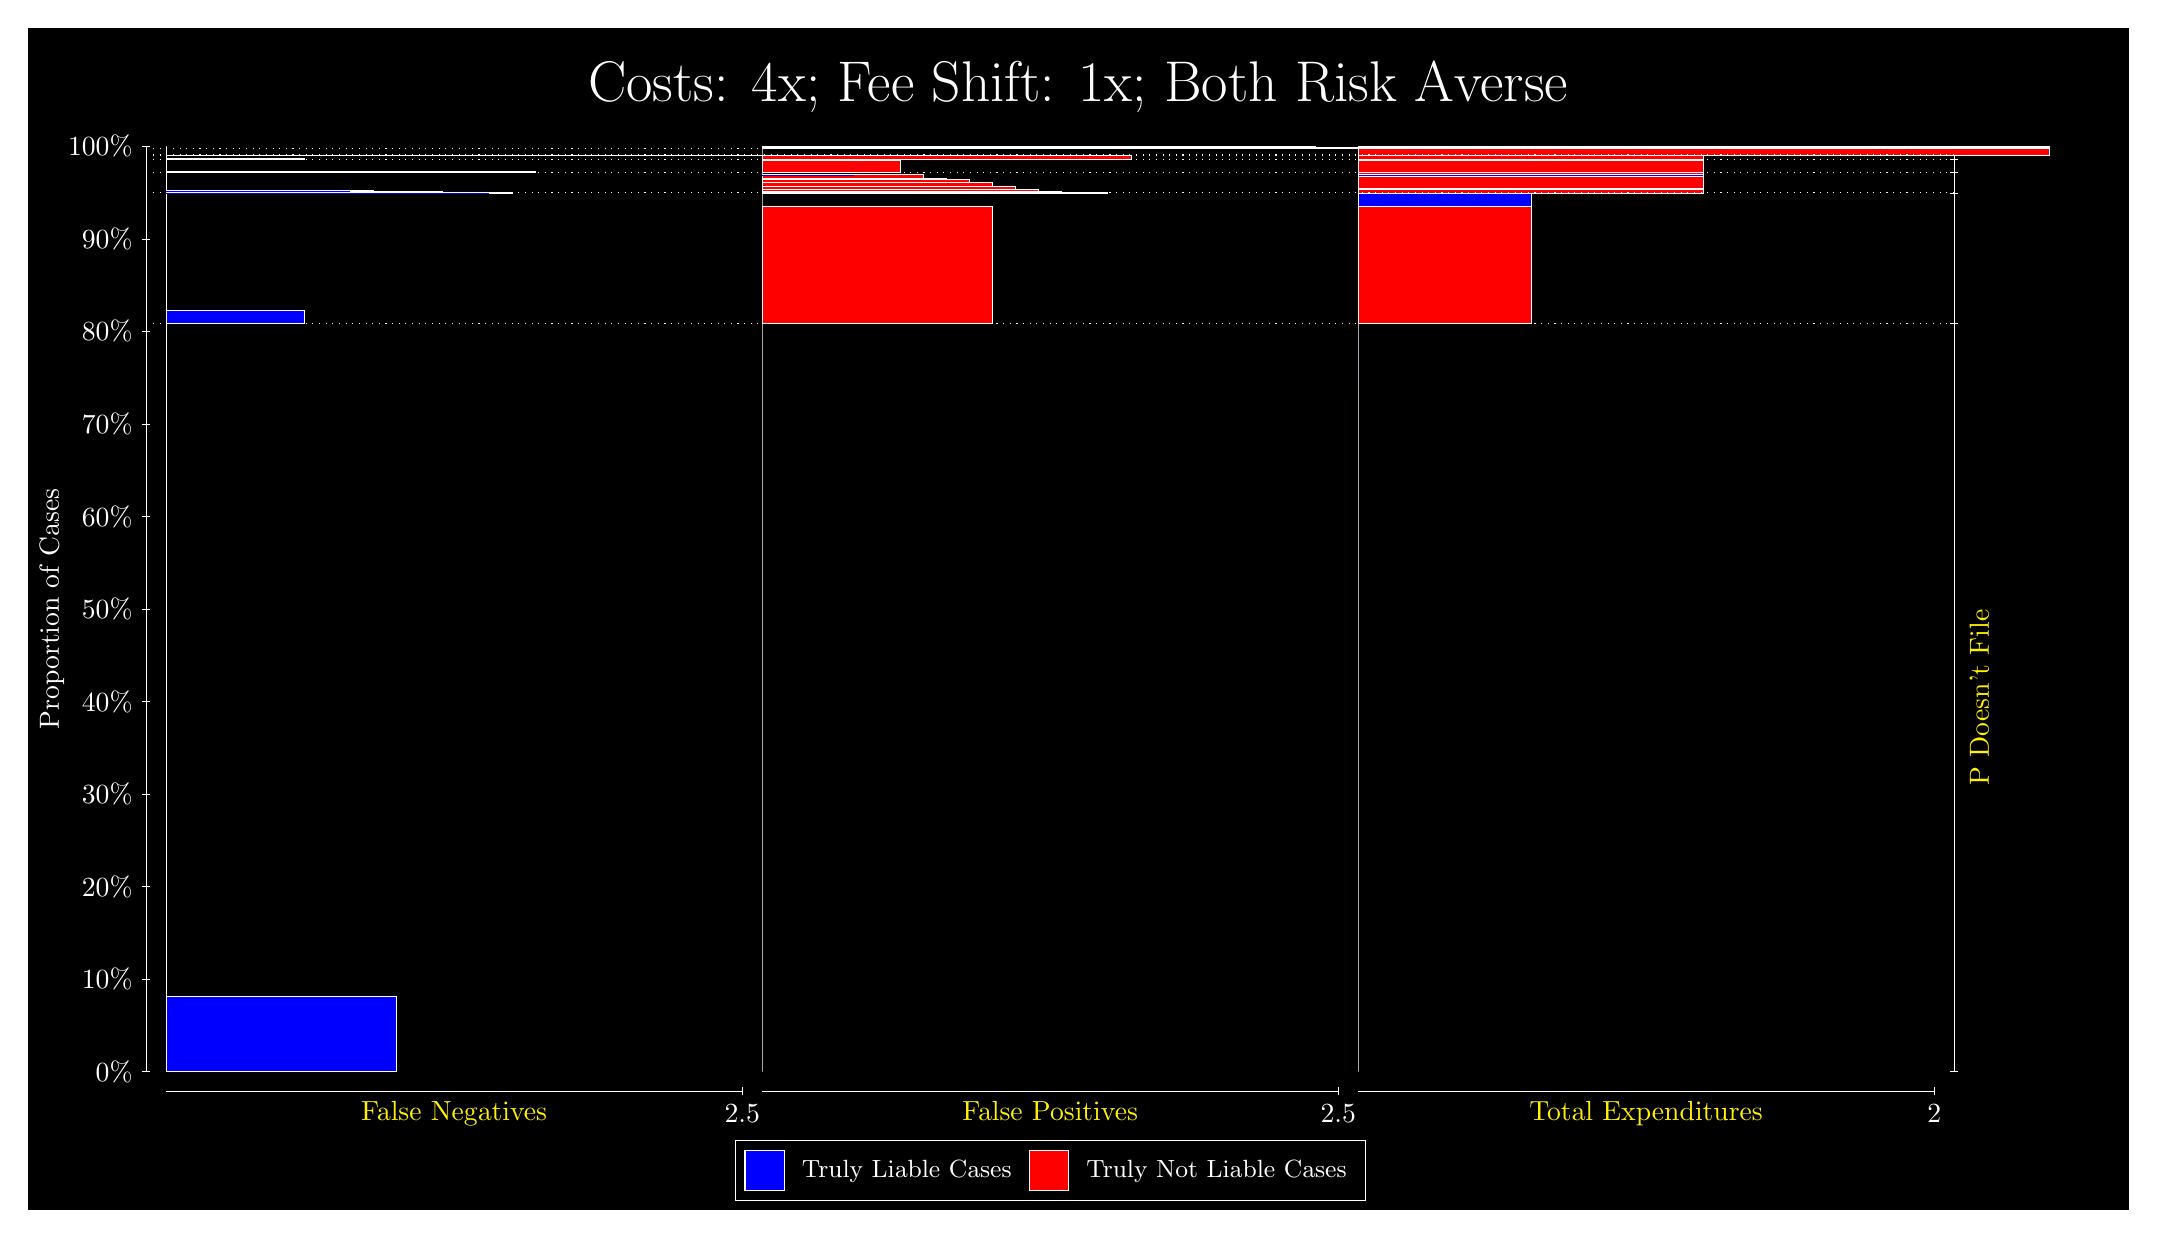
\begin{tikzpicture}
\draw[fill=black] (0,0) rectangle (26.667,15);
\draw[text=white] (0,13.5) rectangle (26.667,15) node[midway] {\huge Costs: 4x; Fee Shift: 1x; Both Risk Averse};
\draw[white, very thin] (1.5,1.75) -- (1.5,13.5);
\node[rotate=90, text=white, anchor=center] at (0.3, 7.625) {Proportion of Cases};
\draw[white, very thin] (1.45,1.75) -- (1.55,1.75);
\node[text=white, anchor=east] at (1.45, 1.75) {0\%};
\draw[white, very thin] (1.45,2.925) -- (1.55,2.925);
\node[text=white, anchor=east] at (1.45, 2.925) {10\%};
\draw[white, very thin] (1.45,4.1) -- (1.55,4.1);
\node[text=white, anchor=east] at (1.45, 4.1) {20\%};
\draw[white, very thin] (1.45,5.275) -- (1.55,5.275);
\node[text=white, anchor=east] at (1.45, 5.275) {30\%};
\draw[white, very thin] (1.45,6.45) -- (1.55,6.45);
\node[text=white, anchor=east] at (1.45, 6.45) {40\%};
\draw[white, very thin] (1.45,7.625) -- (1.55,7.625);
\node[text=white, anchor=east] at (1.45, 7.625) {50\%};
\draw[white, very thin] (1.45,8.8) -- (1.55,8.8);
\node[text=white, anchor=east] at (1.45, 8.8) {60\%};
\draw[white, very thin] (1.45,9.975) -- (1.55,9.975);
\node[text=white, anchor=east] at (1.45, 9.975) {70\%};
\draw[white, very thin] (1.45,11.15) -- (1.55,11.15);
\node[text=white, anchor=east] at (1.45, 11.15) {80\%};
\draw[white, very thin] (1.45,12.325) -- (1.55,12.325);
\node[text=white, anchor=east] at (1.45, 12.325) {90\%};
\draw[white, very thin] (1.45,13.5) -- (1.55,13.5);
\node[text=white, anchor=east] at (1.45, 13.5) {100\%};

\draw[white, very thin] (24.457,1.75) -- (24.457,13.5);
\draw[white, very thin] (24.407,1.75) -- (24.507,1.75);
\node[anchor=west] at (24.407, 1.75) {};
\draw[white, very thin] (24.407,11.252) -- (24.507,11.252);
\node[anchor=west] at (24.407, 11.252) {};
\draw[white, very thin] (24.407,12.909) -- (24.507,12.909);
\node[anchor=west] at (24.407, 12.909) {};
\draw[white, very thin] (24.407,13.168) -- (24.507,13.168);
\node[anchor=west] at (24.407, 13.168) {};
\draw[white, very thin] (24.407,13.334) -- (24.507,13.334);
\node[anchor=west] at (24.407, 13.334) {};
\draw[white, very thin] (24.407,13.39) -- (24.507,13.39);
\node[anchor=west] at (24.407, 13.39) {};
\draw[white, very thin] (24.407,13.477) -- (24.507,13.477);
\node[anchor=west] at (24.407, 13.477) {};
\draw[white, very thin] (24.407,13.5) -- (24.507,13.5);
\node[anchor=west] at (24.407, 13.5) {};

\draw[white, very thin, fill=blue] (1.75,1.75) rectangle (4.6775,2.7002);
\draw[white, very thin, fill=red] (1.75,2.7002) rectangle (1.75,11.252);
\draw[white, very thin, fill=blue] (1.75,11.252) rectangle (3.5065,11.418);
\draw[white, very thin, fill=red] (1.75,11.418) rectangle (1.75,12.909);
\draw[white, very thin, fill=blue] (1.75,12.909) rectangle (6.1413,12.912);
\draw[white, very thin, fill=blue] (1.75,12.912) rectangle (5.8486,12.913);
\draw[white, very thin, fill=blue] (1.75,12.913) rectangle (5.5558,12.919);
\draw[white, very thin, fill=blue] (1.75,12.919) rectangle (5.2631,12.925);
\draw[white, very thin, fill=blue] (1.75,12.925) rectangle (4.9703,12.932);
\draw[white, very thin, fill=blue] (1.75,12.932) rectangle (4.6775,12.934);
\draw[white, very thin, fill=blue] (1.75,12.934) rectangle (4.3848,12.936);
\draw[white, very thin, fill=blue] (1.75,12.936) rectangle (4.092,12.937);
\draw[white, very thin, fill=blue] (1.75,12.937) rectangle (3.7993,12.938);
\draw[white, very thin, fill=red] (1.75,12.938) rectangle (1.75,13.168);
\draw[white, very thin, fill=blue] (1.75,13.168) rectangle (6.4341,13.18);
\draw[white, very thin, fill=red] (1.75,13.18) rectangle (1.75,13.334);
\draw[white, very thin, fill=blue] (1.75,13.334) rectangle (3.5065,13.342);
\draw[white, very thin, fill=red] (1.75,13.342) rectangle (1.75,13.39);
\draw[white, very thin, fill=blue] (1.75,13.39) rectangle (11.704,13.392);
\draw[white, very thin, fill=red] (1.75,13.392) rectangle (1.75,13.477);
\draw[white, very thin, fill=red] (1.75,13.477) rectangle (1.75,13.493);
\draw[white, very thin, fill=blue] (1.75,13.493) rectangle (1.75,13.5);
\draw[white, very thin, fill=red] (9.3189,1.75) rectangle (9.3189,10.302);
\draw[white, very thin, fill=blue] (9.3189,10.302) rectangle (9.3189,11.252);
\draw[white, very thin, fill=red] (9.3189,11.252) rectangle (12.246,12.742);
\draw[white, very thin, fill=blue] (9.3189,12.742) rectangle (9.3189,12.909);
\draw[white, very thin, fill=red] (9.3189,12.909) rectangle (13.71,12.915);
\draw[white, very thin, fill=red] (9.3189,12.915) rectangle (13.417,12.921);
\draw[white, very thin, fill=red] (9.3189,12.921) rectangle (13.125,12.935);
\draw[white, very thin, fill=red] (9.3189,12.935) rectangle (12.832,12.953);
\draw[white, very thin, fill=red] (9.3189,12.953) rectangle (12.539,12.998);
\draw[white, very thin, fill=red] (9.3189,12.998) rectangle (12.246,13.043);
\draw[white, very thin, fill=red] (9.3189,13.043) rectangle (11.954,13.086);
\draw[white, very thin, fill=red] (9.3189,13.086) rectangle (11.661,13.098);
\draw[white, very thin, fill=red] (9.3189,13.098) rectangle (11.368,13.139);
\draw[white, very thin, fill=blue] (9.3189,13.139) rectangle (10.783,13.139);
\draw[white, very thin, fill=blue] (9.3189,13.139) rectangle (10.49,13.14);
\draw[white, very thin, fill=blue] (9.3189,13.14) rectangle (10.197,13.142);
\draw[white, very thin, fill=blue] (9.3189,13.142) rectangle (9.9044,13.144);
\draw[white, very thin, fill=blue] (9.3189,13.144) rectangle (9.6116,13.151);
\draw[white, very thin, fill=blue] (9.3189,13.151) rectangle (9.3189,13.168);
\draw[white, very thin, fill=red] (9.3189,13.168) rectangle (11.075,13.321);
\draw[white, very thin, fill=blue] (9.3189,13.321) rectangle (9.3189,13.334);
\draw[white, very thin, fill=red] (9.3189,13.334) rectangle (14.003,13.382);
\draw[white, very thin, fill=blue] (9.3189,13.382) rectangle (11.075,13.39);
\draw[white, very thin, fill=red] (9.3189,13.39) rectangle (9.3189,13.475);
\draw[white, very thin, fill=blue] (9.3189,13.475) rectangle (9.3189,13.477);
\draw[white, very thin, fill=red] (9.3189,13.477) rectangle (19.273,13.493);
\draw[white, very thin, fill=blue] (9.3189,13.493) rectangle (16.345,13.5);
\draw[white, very thin, fill=red] (16.888,1.75) rectangle (16.888,10.302);
\draw[white, very thin, fill=blue] (16.888,10.302) rectangle (16.888,11.252);
\draw[white, very thin, fill=red] (16.888,11.252) rectangle (19.083,12.742);
\draw[white, very thin, fill=blue] (16.888,12.742) rectangle (19.083,12.909);
\draw[white, very thin, fill=red] (16.888,12.909) rectangle (21.279,12.954);
\draw[white, very thin, fill=blue] (16.888,12.954) rectangle (21.279,12.961);
\draw[white, very thin, fill=red] (16.888,12.961) rectangle (21.279,13.125);
\draw[white, very thin, fill=blue] (16.888,13.125) rectangle (21.279,13.145);
\draw[white, very thin, fill=red] (16.888,13.145) rectangle (21.279,13.165);
\draw[white, very thin, fill=blue] (16.888,13.165) rectangle (21.279,13.168);
\draw[white, very thin, fill=red] (16.888,13.168) rectangle (21.279,13.321);
\draw[white, very thin, fill=blue] (16.888,13.321) rectangle (21.279,13.334);
\draw[white, very thin, fill=red] (16.888,13.334) rectangle (21.279,13.382);
\draw[white, very thin, fill=blue] (16.888,13.382) rectangle (21.279,13.39);
\draw[white, very thin, fill=red] (16.888,13.39) rectangle (25.67,13.475);
\draw[white, very thin, fill=blue] (16.888,13.475) rectangle (25.67,13.477);
\draw[white, very thin, fill=red] (16.888,13.477) rectangle (25.67,13.493);
\draw[white, very thin, fill=blue] (16.888,13.493) rectangle (25.67,13.5);
\draw[white, dotted] (1.5,11.252) -- (24.457,11.252);
\draw[white, dotted] (1.5,12.909) -- (24.457,12.909);
\draw[white, dotted] (1.5,13.168) -- (24.457,13.168);
\draw[white, dotted] (1.5,13.334) -- (24.457,13.334);
\draw[white, dotted] (1.5,13.39) -- (24.457,13.39);
\draw[white, dotted] (1.5,13.477) -- (24.457,13.477);
\draw[white, very thin] (1.75,1.5) -- (9.0689,1.5);
\node[text=yellow, anchor=north] at (5.4094, 1.5) {False Negatives};
\draw[white, very thin] (9.0689,1.45) -- (9.0689,1.55);
\node[text=white, anchor=north] at (9.0689, 1.45) {2.5};

\draw[white, very thin] (9.3189,1.5) -- (16.638,1.5);
\node[text=yellow, anchor=north] at (12.978, 1.5) {False Positives};
\draw[white, very thin] (16.638,1.45) -- (16.638,1.55);
\node[text=white, anchor=north] at (16.638, 1.45) {2.5};

\draw[white, very thin] (16.888,1.5) -- (24.207,1.5);
\node[text=yellow, anchor=north] at (20.547, 1.5) {Total Expenditures};
\draw[white, very thin] (24.207,1.45) -- (24.207,1.55);
\node[text=white, anchor=north] at (24.207, 1.45) {2};

\node[text=yellow, centered, rotate=90] at (24.777, 6.501) {P Doesn't File};







\draw (12.978300999999998,1.5) node[draw=none] (baseCoordinate) {};
\begin{scope}[align=center]
        \matrix[scale=0.5, draw=white, below=0.5cm of baseCoordinate, nodes={draw}, column sep=0.1cm]{
            \node[rectangle, draw, minimum width=0.5cm, minimum height=0.5cm, fill=blue] {}; &
            \node[draw=none, font=\small, text=white] (B) {Truly Liable Cases}; &
            \node[rectangle, draw, minimum width=0.5cm, minimum height=0.5cm, fill=red] {}; &
            \node[draw=none, font=\small, text=white] (B) {Truly Not Liable Cases}; \\
            };
\end{scope}

\end{tikzpicture}
\end{document}